
\item Two rectangular blocks, having identical dimensions, can be arranged either in configuration I or in configuration II as shown in the figure. One of the blocks has thermal conductivity \( \kappa \) and the other \( 2\kappa \). The temperature difference between the ends along the x-axis is the same in both the configurations. It takes 9 s to transport a certain amount of heat from the hot end to the cold end in the configuration I. The time to transport the same amount of heat in the configuration II is
\begin{center}
    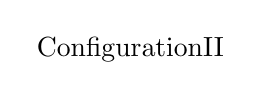
\begin{tikzpicture}
        \node at (0, 0){ConfigurationII};
    \end{tikzpicture}
\end{center}
\begin{tasks}(2)
    \task \( 2.0 \) s
    \task \( 3.0 \) s
    \task \( 4.5 \) s
    \task \( 6.0 \) s
\end{tasks}
